\section{Processer}

För att kunna leverera anpassat webbinehåll till besökaren av en webbsida, måste systemet ha ett sätt att om denne kunna identifiera information. SmartElement använder sig av några olika tekniker för att samla in information om besökare då de anländer på en webbsida, dels teknisk information och dels statistik.

Denna information används sedan för att söka igenom tillgängligt innehåll och testa om informationen passar för de filter som registrerats. Filtren bygger i sig på olika villkor som kan appliceras på den insamlade informationen.

\subsection{Information om besökaren}

SmartElement använder sig till stor del av statistik som systemet samlar ihop med hjälp av en JavaScript tag som körs i besökarens webbläsare då denne besöker en sida som använder systemet. Denna information skickas till back-endsystemet som vidare processerar datan och sparar den i en dokumentdatabas under ett besökarobjekt. På detta vis kan systemet komma ihåg besökare mellan sessioner och på så vis skapa historik om dennes beteende och vanor, vilket i sin tur är till nytta för att hitta det bästa innehållet att presentera.

\subsubsection{Hänvisningsinformation}

\begin{figure}[h!]
\centering
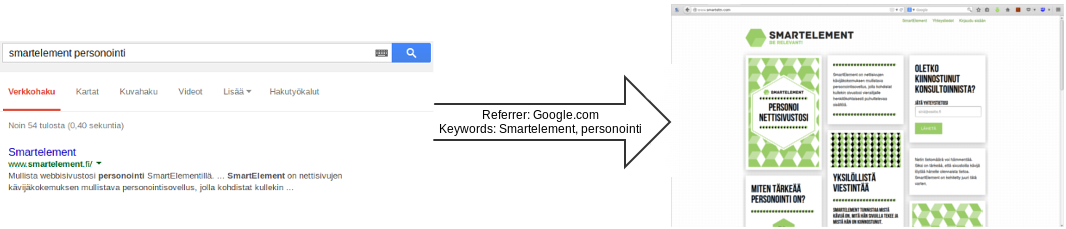
\includegraphics[width=150mm]{assets/images/smelereferer.png}
\caption{Hänvisningsinformationen berättar varifrån beökaren kommer}
\label{referer}
\end{figure}

Den första informationen som registreras om besökaren är varifrån denne anländer till sidan. Webbläsare skickar oftast en s.k. referer variabel när man navigerar till en webbsida genom att klicka på en länk. Denna variabel innehåller adressen på sidan som visade länken.

Genom att spara denna information får man dels en indikation av varifrån en besökare hittar till sidan, men även en indikation av vilken typs sidor den aktuella besökaren ofta besöker.

En nackdel är att hänvisningsinformation inte alltid finns tillgänglig. Avsaknad av denna information leder till att ett definitivt svar inte erhålls om hur besökaren hittat till sidan. Detta sker på grund av att hänvisningsinformation inte skickas t.ex. när man navigerar till webbsidan från en sida med krypterad anslutning, om besökarens webbläsare har konfigurerats att inte sända informationen eller om besökaren helt enkelt skrivit in webbsidans adress i sin webbläsare och är en så kallad direkt träff. \citep{httprfc}

\subsubsection{IP Geolokalisering}

\begin{figure}[h!]
\centering
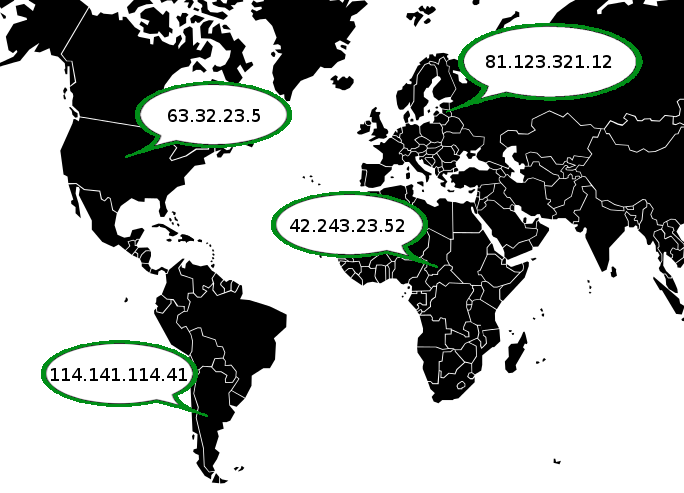
\includegraphics[width=120mm]{assets/images/geolocation.png}
\caption{IP-geolokalisering handlar om att associera plats med IP-address}
\label{geolocation}
\end{figure}

Nästa information som samlas in om besökaren är en uppskattning av dennes position på basis av den information som registrerats för IP-adressen som förfrågan kommer från.

SmartElement använder sig av en databas som köps in av ett företag som specialiserar sig på att upprätthålla så noggrann information som möjligt om var i världen IP-adresser egentligen är registrerade. Från denna databas söker systemet sedan fram information om besökarens läge. Information som är tillgänglig är bland annat vilket land besökaren befinner sig i, vilken region inom landet samt vilken stad.

Trots att informationen i databasen är av rätt hög kvalitet, kan man inte helt och hållet lita på information som genereras genom IP-geolokalisering. Dels så är IP-addressen som sänds till servern inte nödvändigtvis besökarens egna IP-address då denne kan vara uppkopplad via en VPN-anslutning eller eventuellt använda sig av en proxy-server som inte vidareförmedlar ursprungsadressen. Detta betyder i sin tur att man får platsen var VPN- eller proxy-serverns IP är registrerad. Ett annat problem är att den information som finns tillgänglig beror på vad besökarens Internet-operator rapporterar. Även om IP-adressen är besökarens egna så kan leverantören ha registrerat adressen på en annan plats än den var besökaren befinner sig. 

\subsubsection{Besökarstatistik}

För varje sidvisning på en webbsida med SmartElement sparas det statistik. Besökarobjektet som sparas i systemet innehåller information om hur ofta besökaren varit på webbplatesen, hur många sidor denne besökt inom webbplatsen, samt hur ofta denne sett en specifik sida.

Genom att skapa statistik som är kopplad till beökaren kan man generera information om besökarens beteende då denne använder webbsidan. Man kan räkna hur ofta denne besöker specifika delar av sidan, om denne inte sett en viss sida på länge, om denne börjat besöka en specifik del mer eller mindre o.s.v. All denna information kan hjälpa att söka fram information som kan tänkas vara relevant för besökaren.

De största problemen med statistik är att den är beroende av möjligheten att identifiera besökaren då denne återvänder till webbsidan. Som systemet är byggt för tillfället hänger detta på användningen av kakor som innehåller ett unikt id-nummer, vilket betyder att systemet tappar besökaren så fort denne raderar denna kaka. Det finns sätt att rundgå detta genom att använda sig av till exempel caching information för att identifiera besökare trots att denne raderat eller blockerat kakor. \citep{ashkanblog}



\subsubsection{Tid}

Vid varje sidvisning registreras tiden för besöket på basis av den tid som besökarens webbläsare rapporterar. Utöver tiden för sidvisningen så beräknar javascript-tagen hur lång tid besökaren spenderat på sidan under det pågående besöket.

Valet att registrera tiden som rapporteras av webbläsaren gjordes för att undvika problem med olika tids-zoner och för att det är troligare att man vill göra ett beslut utgående från besökarens tid, och eftersom tagen registrerar besökarens tid så får systemet samtidigt möjligheten att registrera besökets längd.

\subsubsection{Användardefinierad information}

För att tillåta så flexibel användning som möjligt, tillåter SmartElement även att upprätthållaren av en webbsida själv definierar information som skickas till servern för processering. Detta sker genom att upprätthållaren lägger till egna dataelement i tagen då den inkluderas på sidan.

Genom att förse tagen med egen information kan upprätthållaren av en webbsida använda information som SmartElement inte i sig kan ta reda på, information som besökaren matar in på webbsidan eller information som uppräthållaren genererar.

Det går även att skapa statistik över användardefinierad information. Funktionen är den samma som för SmartElements egna statistik, man kan lägga till nya värden för varje sidvisning och sedan göra filtrering baserad på denna informationssamling.

Genom denna teknik kan upprätthållaren i princip använda vad helst information som är relevant i dennes fall. Exempel på data som kunde vara intressant att spara är shoppingvagnens innehåll i en webbutik, någon form av id för registrerade användare, aktiva kampanjer och annan information om webbsidans status vid sidvisningen. Systemet sätter ingen begränsning på vad som skickas förutom att det måste sändas i formen av en samling av värden med nycklar.

\subsection{Filtrering}


För att välja ut vilket innehålls-element som skall skickas till besökaren, använder sig systemet av informationen som samlats in och ett eller flera filter som upprätthållaren av webbsidan definierat för de olika elementen som registrerats i systemet. Filtersystemet bygger på användningen av enkla test som i kombination med olika typers data bildar en fråga om en besökare.

\subsubsection{Villkor}

I grunden bygger SmartElements filtersystem på 12 enkla villkorsfunktioner som utför en jämförelse mellan den information tagen skickat och den information som upprätthållaren sparat i filtret.

De tolv villkoren som kan användas samt de datatyper de kan hantera visas i Tabell \ref{table:villkor}.

\begin{table}
    \begin{tabular}{|l|p{8cm}|l|}
    \hline
    Namn & Funktion & Datatyp \\
    \hline
    Större än & Testar om värdet är större än det i filtret & Alfanumerisk \\
    \hline
    Mindre än & Negation av större än villkoret & Alfanumerisk \\
    \hline
    Lika med & Testar om värdet är lika med det i filtret & Godtycklig \\
    \hline
    Inte lika med & Negation av lika med villkoret & Godtycklig \\
    \hline
    I samling & Testar om samlingen som registrerats i filtret innehåller värdet som sänts & Samling \\
    \hline
    Icke i samling & Negation av "i samling" villkoret & Samling \\
    \hline
    Innehåller & Testar om värdet i filtret innehåller värdet som sändts & Text \\
    \hline
    Innehåller ej & Negation av innehåller-villkoret & Text \\
    \hline
    Börjar med & Testar om värdet som skickats börjar med värdet i filtret & Text \\
    \hline
    Slutar med & Testar om värdet som skickats slutar med värdet i filtret & Text \\
    \hline
    Tom & Testar om värdet som skickats är tomt & Text, Samling \\
    \hline
    Icke tom & Negation av tomhetsfiltret & Text, Samling \\
    \hline
    \end{tabular}
    \caption{Villkorstyper}
    \label{table:villkor}
\end{table}

Genom att kombinera dessa enkla villkor med den data som samlas in vid sidvisningar skapas filter som kan göra meningsfulla beslut om besökaren.

Under utvecklingen av SmartElement utvaldes några färdiga filtrerings-metoder för implementering i systemet som en grund för upprätthållare att börja bygga sin anpassning. Genom att studera den tillgängliga informationen valdes några frågor ut som var lätta att identifiera. Dessa utgör de inbyggda filtren i SmartElement.

\subsubsection{Stadsfiltret}

Stadsfiltret använder sig av informationen som samlats in genom IP-geolokalisering och tillåter upprätthållaren att visa specifikt innehåll för besökare från en viss stad.

Motivationen för att implementera stadsfiltret kom från ett användningsfall var upprätthållaren kan köra kampanjer för olika kontor i olika städer eller visa kontorsspecifika öppethållningstider.

\subsubsection{Landfiltret}

Landsfiltret använder sig av IP-geolokaliseringsinformationen för att tillåta upprätthållaren att avgränsa innehåll på basis av vilket land besök kommer ifrån.

Motivationen bakom landsfiltret var att tillåta dels större företag, som sträcker sig över landsgränser, att visa landsspecifik information på sin webbsida, samt mindre företag att välja att visa mera specifik information för inhemska besökare, och en mera generell information för internationella besökare.

\subsubsection{Datumfiltret}

Datumfiltret använder sig av dagens datum för att tillåta upprätthållaren att specificera när ett innehåll skall visas. Filtret kan användas med de olika jämförelse-villkoren. Upprätthållaren kan specificera ett datum efter vilket innehåll skall visas eller ett datum före vilket det skall visas. Med lika med villkoret kan man specificera en enda dag då innehållet skall visas och lika så en specifik dag då det inte skall visas.

Motivationen bakom datumfiltret var att ge upprätthållaren möjligheten att visa kampanj innehåll under en specifik tid genom att kombinera två datum filter, ett med en nedre gräns och ett med en övre.

\subsubsection{Dagsfiltret}

Dagsfiltret använder sig även av datumet för filtrering. Till skillnad från datumfiltret så tar dagsfiltret emot en samling av dagar då ett innehåll skall visas. Filtret kan antingen inkludera dagar eller exkludera dagar.

Användningsfallet som ledde till dagsfiltret var att en upprätthållare vill visa en tabell med öppettider under veckan men ett anpassat element under veckoslutet som föreslår att besökaren gör en beställning genom en webb-butik.

\subsubsection{Besökstidsfiltret}

Besökstidsfiltret använder sig av tiden en besökare spenderat på webbsidan för att filtrera innehåll. Filtret använder de olika jämförande villkoren för att tillåta upprätthållare att visa innehåll för besökare som spenderat en specifik tid på sidan. Man kan ställa in en nedre gräns, en övre gräns och även en exakt tid då innehåll skall visas eller döljas.

Användningsfallen för besökstidsfiltret var att upprätthållaren vill skapa ett element som visar ett specialerbjudande för besökare som har spenderat en längre tid på webbsidan men inte beställt något samt att upprätthållaren vill visa nyheter för besökare som nyss anlänt.

\subsubsection{Nyckelordsfiltret}

Nyckelordsfiltret använder sig av hänvisningsinformationen för att filtrera ut vilka nyckelord som använts i en sök-motor om besökaren nått sidan via en sådan. Filtret tillåter upprätthållaren att specificera grupper av nyckelord som antingen skall eller inte skall vara bland de som använts.

Användningsfallet bakom nyckelordsfiltret är att en upprätthållare väljer att lyfta fram speciell information som passar in på den webbsökning som besökaren använt för att hitta till webbplatsen.

\subsubsection{Landningssidefiltret}

Landningssidefiltret använder sig av statistikinformationen för att välja ut anpassat innehåll. Funktionaliteten fungerar genom att jämföra den första sidan under det aktiva besöket mot en samling av sidor som den antingen skall eller inte skall finnas bland.

Användningsfallet för landningssidefiltret är att en upprätthållare använder sig av en marknadsföringswebbadress som leder till en speciell sida. Efter detta kan elementen på sidan återspegla kampanjen.

\subsubsection{Sidantalsfiltret}

Sidantalsfiltret använder sig av statistikinformationen för att ge upprätthållaren möjlighet att skapa filter som använder antalet av sidor som visats under det aktiva besöket för att visa eller dölja innehåll.

Användningsfallet för sidantalsfiltret är en upprätthållare som vill visa ett element som ändrar med antalet sidor som visats och på så vis ger information som passar med besökarens bekantskap med sidan och på samma gång ger en levande bild av informationen.

\subsubsection{Hänvisarfiltret}

Hänvisarfiltret använder sig av hänvisningsinformationen för att tillåta upprätthållare att skapa filter som agerar på grupper av hänvisare och på så vis tillåter innehåll att kopplas till de sidor som sänt besökaren till webbsidan.

Användningsfallet för hänvisarfiltret är att upprätthållaren vill skapa ett element som visar speciellt innehåll för besökare som når dennes webbsida genom en av deras samarbetspartners.

\subsubsection{Regionsfiltret}

Regionsfiltret använder sig av IP-geolokaliseringsinformation för att tillåta upprätthållaren att visa innehåll anpassat till besökarens region. I Finland kan man t.ex. specificera att ett innehåll skall visas endast om besökaren befinner sig i södra Finland.

Användningsfallet är att upprätthållaren har regionalkampanjer som använder samma element på sidan för att visa relevanta information på basis av var besökaren befinner sig.

\subsubsection{Tidsfiltret}

Tidsfiltret använder den aktuella tiden för att välja ut vilket innehåll som skall visas. Upprätthållaren kan skapa filter utgående från villkoren större än, mindre än, lika med och icke lika med för att skapa filter som visar olika innehåll olika tider av dagen.

Användningsfallet för tidsfiltret är att upprätthållaren vill visa speciell information när en butik är öppen, när den håller på att stänga och när den är stängd.

\subsubsection{Besöksfiltret}

Besöksfiltret använder sig av statistikinformationen för att tillåta filtrering baserat på antalet besök som gjorts till webbsidan. Med hjälp av större än, mindre än, lika med och icke lika med villkoren kan upprätthållaren skapa filter som visar innehåll på basis denna statistik.

Användningsfallet för besöksfiltret är att upprätthållaren vill visa information som passar besökarens lojalitet till webbsidan. En besökare som ofta återkommer kan se ett innehåll som reflekterar detta.

\subsubsection{Anpassningsbart filter}

Den sista filterklassen är det anpassningsbara filtret vilket tillåter upprätthållaren att skapa filter helt baserat på sina egna behov. Filtret tillåter användning av godtycklig villkorsfunktion med godtycklig data. Beroende på vilken villkorsfunktion som konfigureras kan det uppstå begränsningar på vilken typs data som kan användas för filtrering. Detta filter ger SmartElement möjligheten implementera ny filtreringsfunktionalitet genom konfiguration.

Användningsfallet för det anpassningsbara filtret är att upprätthållaren kan skapa ett filter helt på basis av sina egna behov genom att specificera vilken data som skall användas och hur den skall användas vid filtrering.

% vim: set tw=78:ts=2:sw=2:et:fdm=marker:wrap:wm=78:ft=tex
% vim: spell spelllang=sv
